\documentclass{beamer}
%\usetheme{Boadilla}
\usetheme{Darmstadt}
%\usetheme{Berkeley}
%\usetheme{Berlin}
%\usetheme{Copenhagen}
%\usetheme{Warsaw}

\DeclareMathOperator*{\argmax}{arg\,max} % Jan Hlavacek
\usepackage{comment} % for block commenting (\begin{comment})
\defbeamertemplate{footline}{left page number}
{%
  %\hspace*{\fill}%
  \hspace*{0.5cm}%
  \usebeamercolor[fg]{page number in head/foot}%
  \usebeamerfont{page number in head/foot}%
  \insertpagenumber\,/\,\insertpresentationendpage%
  \hspace*{\fill}\vskip2pt%
}
\setbeamertemplate{footline}[left page number]

\title{Developing Strategies with Reinforcement Learning}
\subtitle{FCOS Short Version}
\author{Cdt Koen Boeckx, Ir}
\date{April 27, 2020}

\begin{document}
\setbeamertemplate{caption}{\raggedright\insertcaption\par} % removes 'Figure:' in figure captions

\begin{frame}
\titlepage
\end{frame}

\begin{frame}{Outline}
\tableofcontents
\end{frame}

\section{Introduction}

\begin{frame}
\frametitle{The IRIS Project}
\begin{block}{Intelligent Recognition Information System}
\begin{itemize}
    \item Piloted by \emph{John Cockerill Defence}
    \item Funding provided by Walloon government
    \item Crews of armoured vehicles are small and do need to process a lot of information about the environment
    \item Goal: develop a pipeline from observation to action suggestion on board of armoured vehicles
    %\item I've worked on strategy development
\end{itemize}
\end{block}
\begin{figure}[htp]
    \centering
    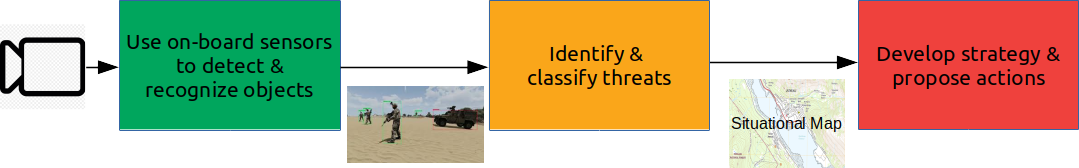
\includegraphics[width=11cm]{images/IRIS_schematic.png}
\end{figure}
\end{frame}

\begin{frame}
\frametitle{Goals of my thesis}
\begin{block}{1. Battlefield Modelling}
\begin{itemize}
    \item An algorithm that simulates a real environment
    \item Simple enough to use
    \item Realistic enough to be useful
\end{itemize}
\end{block}
\pause
\begin{block}{2. Develop strategies}
\begin{itemize}
    \item Use \emph{Reinforcement Learning} to develop strategies
    \item Assess performance of different RL algorithms
    \item Use battlefield model to generate episodes
\end{itemize}
\end{block}
\end{frame}

\section{Reinforcement Learning}
\begin{frame}
\frametitle{Reinforcement Learning}
\begin{columns}
\column{0.5\textwidth}
\begin{alertblock}{Reinforcement Learning}
\begin{itemize}
    \item Learn a policy $\pi$ through interaction with environment
    \item Policy $\pi(a | s)$: given state $s$, returns action $a$
    \item No explicit examples, just a reward signal
\end{itemize}

\end{alertblock}
\begin{figure}[htp]
    \centering
    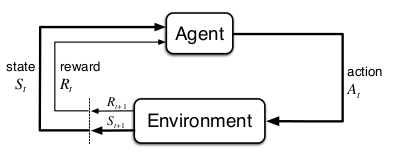
\includegraphics[scale=0.4]{images/mdp.png}
\end{figure}
\column{0.5\textwidth}
\begin{block}{Markov Decision Process}
\begin{itemize}
    \item Only state is needed to encode all information
    \item Agent takes actions based on state
    \item Based on action, the environment changes state and returns reward
    \item Goal: maximize cumulative reward $G_t$
    \begin{equation*}
        G_t &= \sum_{k=0}^{\infty} \gamma^k R_{t+k+1}
    \end{equation*}
\end{itemize}
\end{block}
\end{columns}
\end{frame}

\begin{frame}
\frametitle{Reinforcement Learning}
\begin{block}{Value approximation}
\begin{itemize}
    \item Estimate the value $Q(s,a) $ of taking action $a$ in state $s$
    \item Derive a policy from this estimated value: $\pi_{*}(s) = \argmax_{a} Q(s, a)$
    \item \emph{Q-learning}: derive $Q(s,a)$ with \emph{Bellman equation}
\end{itemize}
\end{block}

\begin{block}{Policy approximation}
\begin{itemize}
    \item Learn the optimal policy $\pi_{*}$ directly
    \item Policies are determined parameters $\theta$
    \item Update the policy parameters with the \emph{policy gradient theorem}
    %\item $\bm{\theta}_{t+1} = \bm{\theta}_t + \alpha \, G_t \, \frac{\nabla_{\bm{\theta}_t} \pi(A_t|S_t, \bm{\theta}_t)}{\pi(A_t|S_t, \bm{\theta}_t)}$
    \item {\tt REINFORCE}, Actor-Critic
\end{itemize}
\end{block}
\end{frame}

\begin{frame}
\frametitle{Deep Reinforcement Learning}
\begin{block}{Problem}
    \begin{itemize}
    \item Classical RL algorithms work with tables that store $Q$-values or policies
    \item This is no longer feasible when the state space becomes large
    \begin{itemize}
        \item Table too large
        \item Can't explore each state
    \end{itemize}
     \end{itemize}
\end{block}
\pause
\begin{block}{Solution}
    \begin{itemize}
    \item Work with function approximators $f(s; \theta)$
    \begin{itemize}
        \item Store weights $\theta$
        \item Generalize beyond encountered states
    \end{itemize}
            
    \item \alert{Deep Learning}: artificial neural networks as function approximators
    \end{itemize}
\end{block}
\end{frame}

\begin{frame}
\frametitle{Deep Learning}
\begin{columns}
\column{0.5\textwidth}
\begin{figure}[htp]
    \centering
    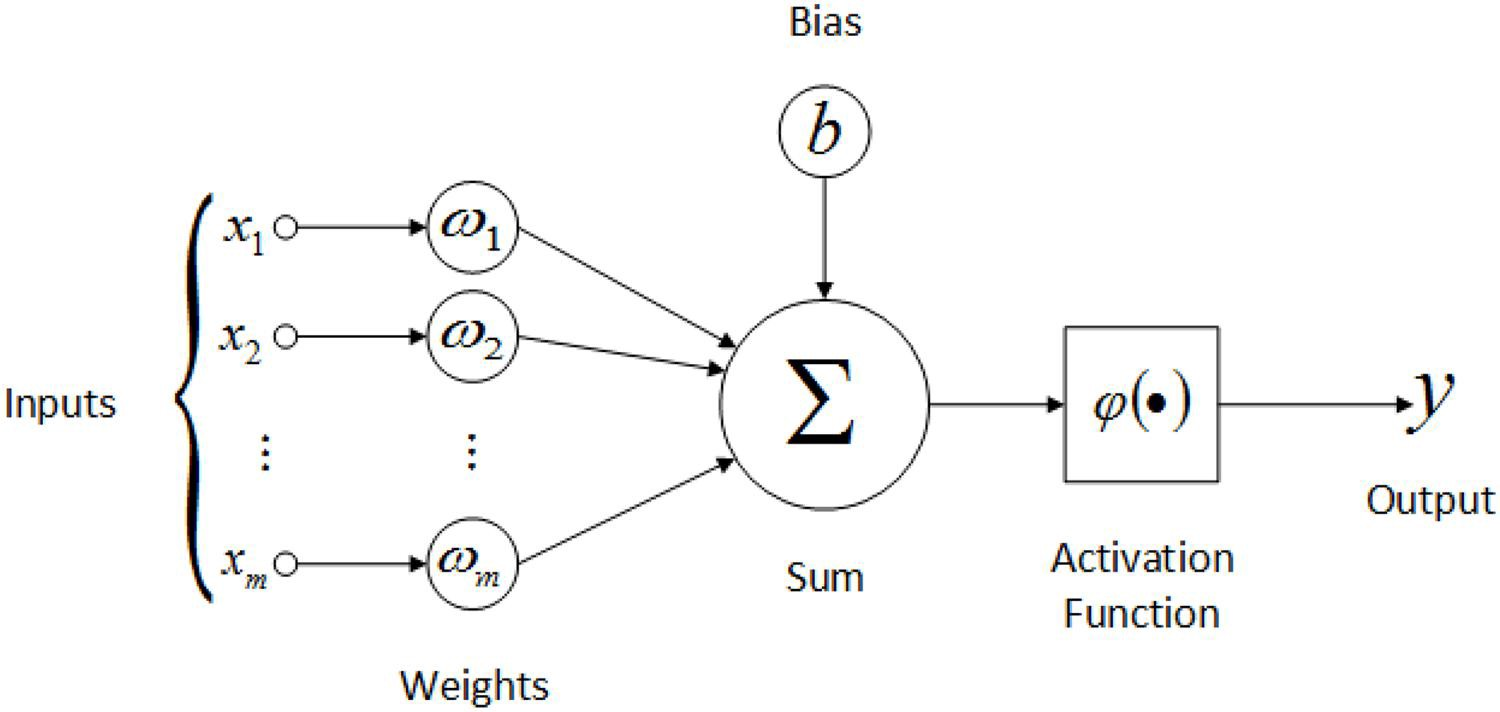
\includegraphics[scale=0.1]{images/neuron.jpeg}
    \caption{An artificial neuron}
\end{figure}
\column{0.5\textwidth}
\begin{figure}[htp]
    \centering
    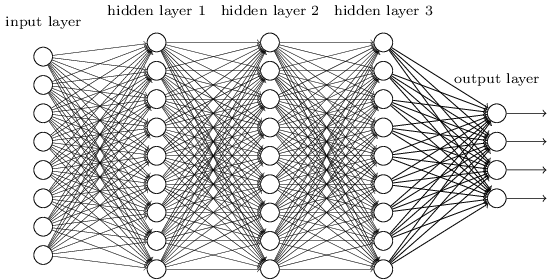
\includegraphics[scale=0.3]{images/neural_net.png}
    \caption{A neural network}
\end{figure}
\end{columns}
\end{frame}

\begin{frame}
\frametitle{Deep Reinforcement Learning}
\begin{block}{Deep Q-networks}
\begin{itemize}
    \item Use a neural net to estimate the value of a state $S$
    \item Loss function $\mathcal{L} = \big [ \color{red} R_t + \gamma \max_{A'} Q(S_{t+1}, A';\, \bm{\theta}) \color{black} - \color{blue} Q(S_t, A_t) \color{black}; \theta \big ]^2$
\end{itemize}
\end{block}
\begin{block}{Deep Policy Gradients}
\begin{itemize}
    \item Use a neural net to represent a policy
\end{itemize}
\begin{figure}[htp]
    \centering
    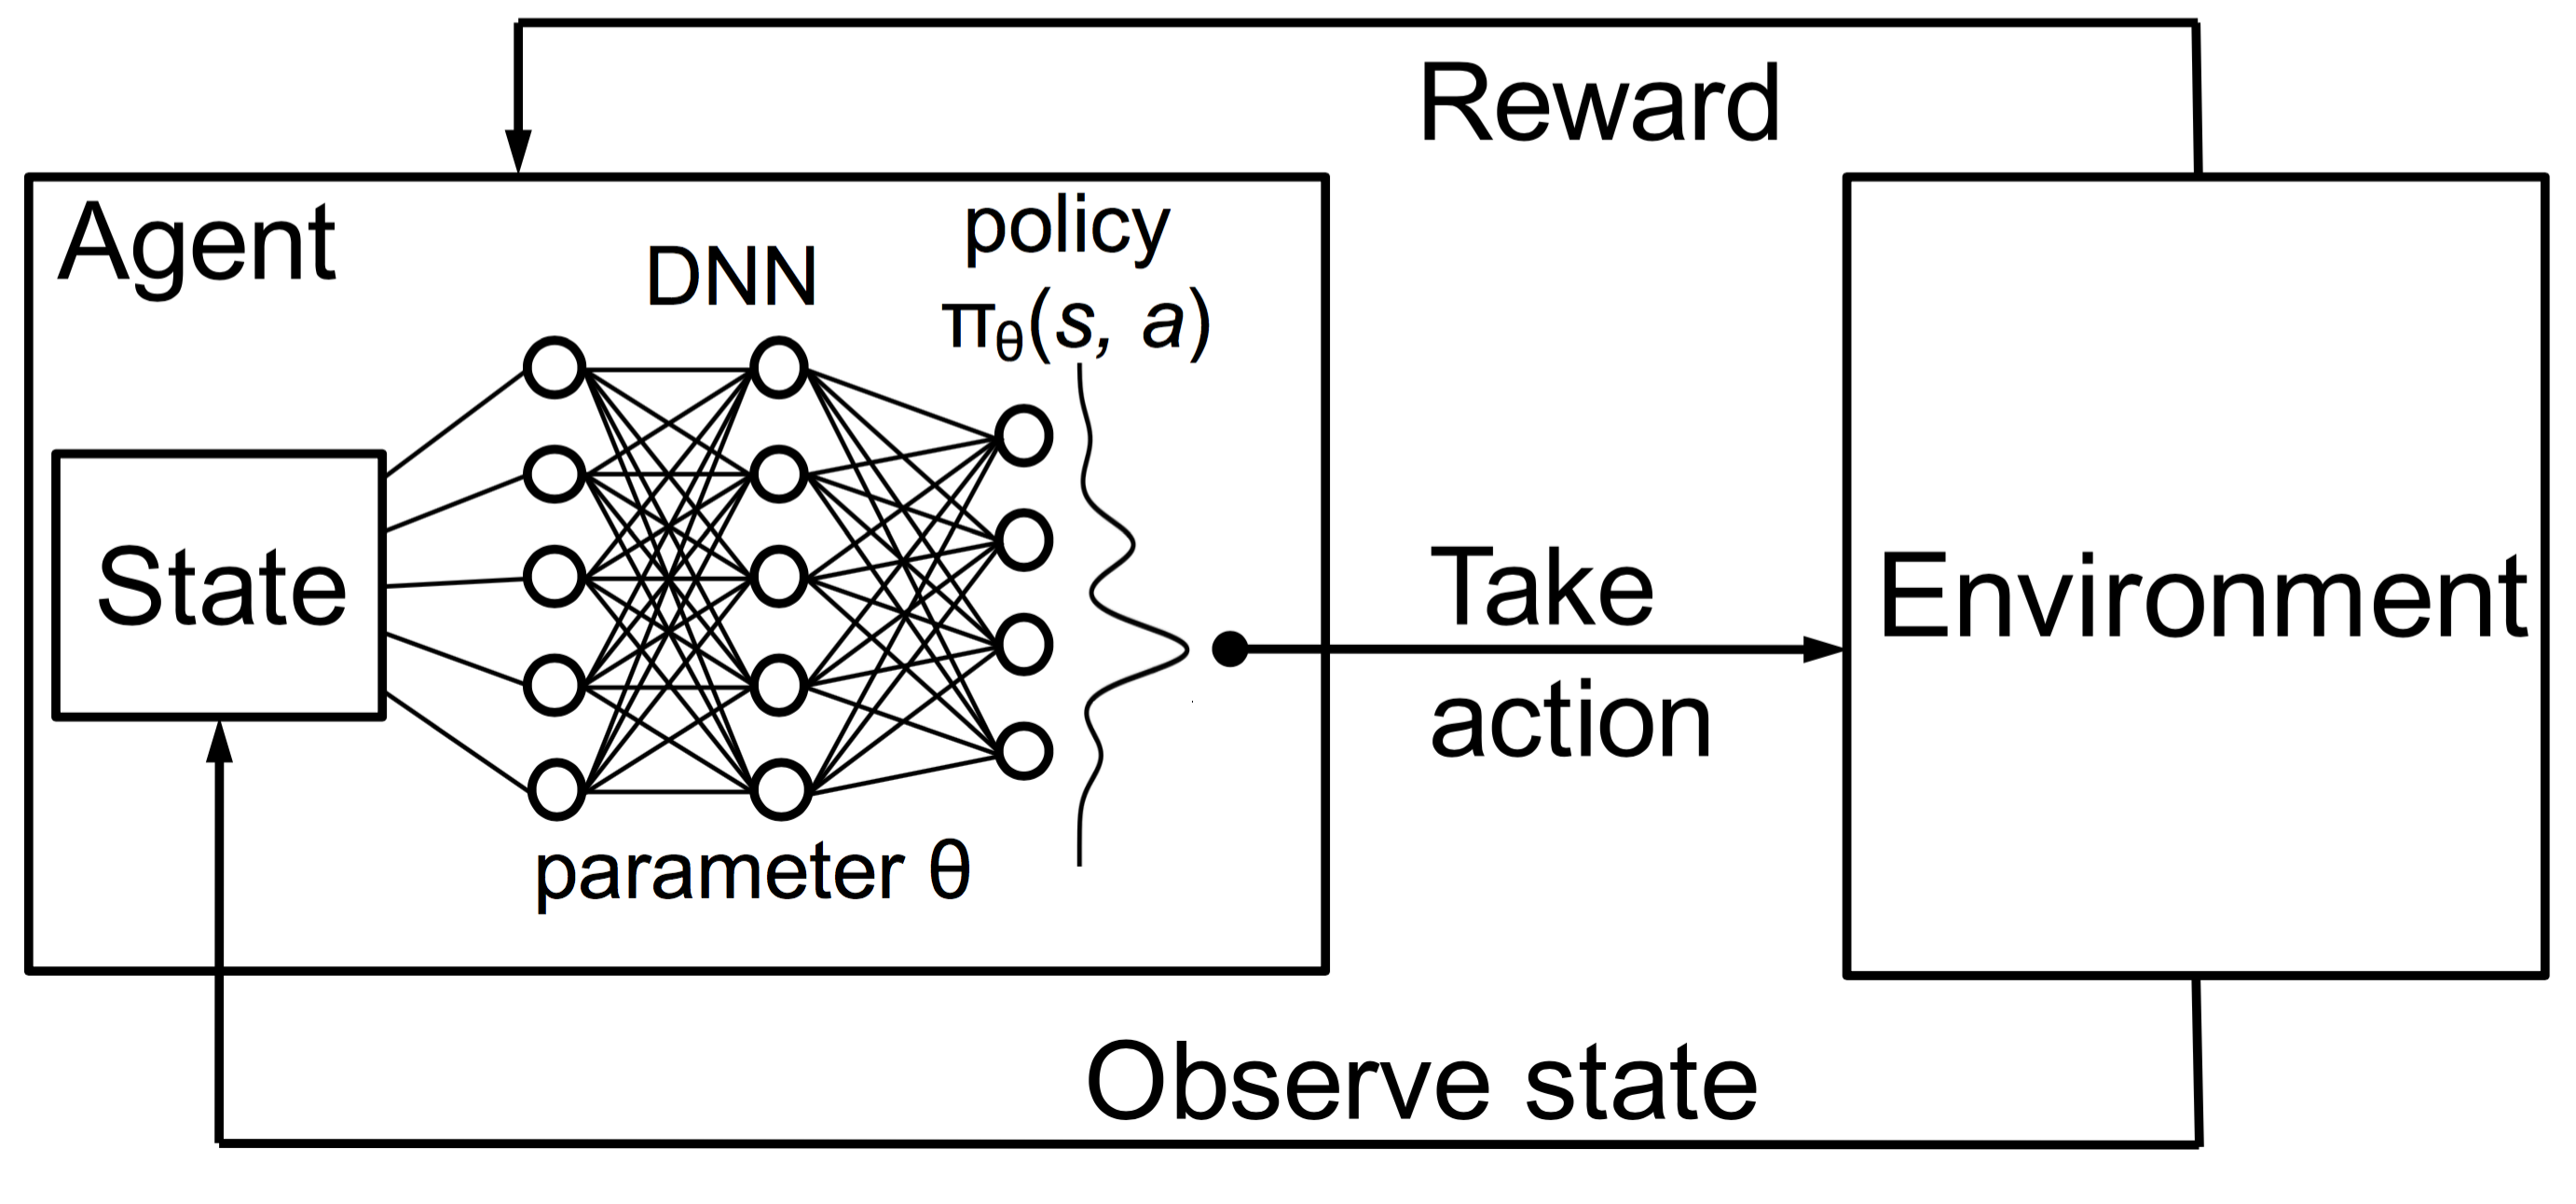
\includegraphics[width=6cm]{images/deep_pg.png}
\end{figure}
\end{block}
\end{frame}

\begin{frame}
\frametitle{Multi-Agent Learning}
\begin{itemize}
    \item Extension of MDP framework
    \item Multiple adaptive agents are present
    \item The agents receive a single, common reward, based on their joint actions
    \item Allows for emergent strategies, but difficult to train
    \item \emph{Credit assignment}: which agent deserves the credit for the win
\end{itemize}
\end{frame}

\begin{frame}
\frametitle{Multi-Agent Learning Algorithms}
\begin{block}{Independent Agents}
\begin{itemize}
    \item Just assumes all agents are independent
    \item Use single-agent algorithm for each agent
    \item $+$ : simple extension of single-agent RL
    \item $-$ : no cooperation between agents
    \item IQL, IAC
\end{itemize}
\end{block}
\begin{block}{QMix}
\begin{itemize}
    \item True multi-agent algorithm
    \item Centralised learning - Decentralised execution
    \item Compute $Q_{tot} = f(Q_1, \dots, Q_N)$ such that $\frac{\partial Q_{tot}}{\partial Q_i} \geq 0$
\end{itemize}
\end{block}
\end{frame}

\begin{frame}
\frametitle{QMix}
\begin{block}{QMix}
\begin{itemize}
    \item True multi-agent algorithm, based on Q-learning
    \item Centralised learning - Decentralised execution
    \item Compute $Q_{tot} = f(Q_1, \dots Q_N)$ such that $\frac{\partial Q_{tot}}{\partial Q_i} \geq 0$
\end{itemize}
\end{block}
\begin{figure}[htp]
    \centering
    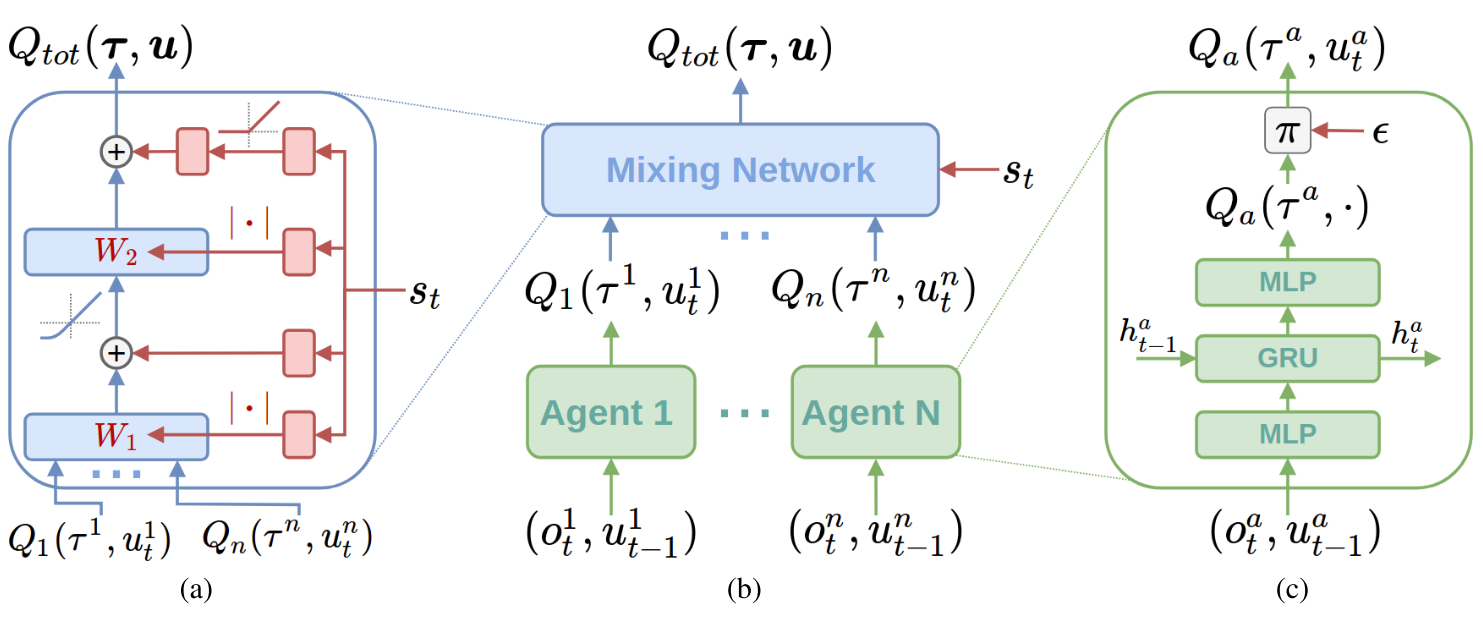
\includegraphics[scale=0.2]{images/qmix_structure.png}
\end{figure}
\end{frame}

\section{Modelling the battlefield}
\begin{frame}{Modelling the battlefield}
\begin{block}{An algorithmic model - What}
\begin{itemize}
    \item A piece of software that simulates a battlefield
    \begin{itemize}
        \item Environment $\leftrightarrow$ Agents
        \item Terrain contains obstacles that block visibility and movement
    \end{itemize}
    \item Goal:
    \begin{itemize}
        \item Generate episodes to train on
        \item Simplifications become explicit
    \end{itemize}
\end{itemize}
\end{block}
\end{frame}


\begin{frame}{Modelling the battlefield}
\begin{block}{An algorithmic model - How}
\begin{itemize}
    \item Each agent can take certain actions: {\tt move}, {\tt aim}, {\tt fire}, \ldots
    \item Agents can shoot at one another; if in range $\rightarrow$ kill
    \item The environment enforces constraints:
        \begin{itemize}
            \item Don't fire when not aiming
            \item Don't fire when opponent is not visible
            \item Don't pass through obstacles
            \item \ldots
        \end{itemize}
    \item The environment takes the actions of the agents and changes state.
    \item Afterwards, the environment returns an \emph{observation} to agents
    \item Team wins if all opposing agents are dead
\end{itemize}
\end{block}
\end{frame}

\begin{frame}{Modelling the battlefield}
\begin{figure}[htp]
    \centering
    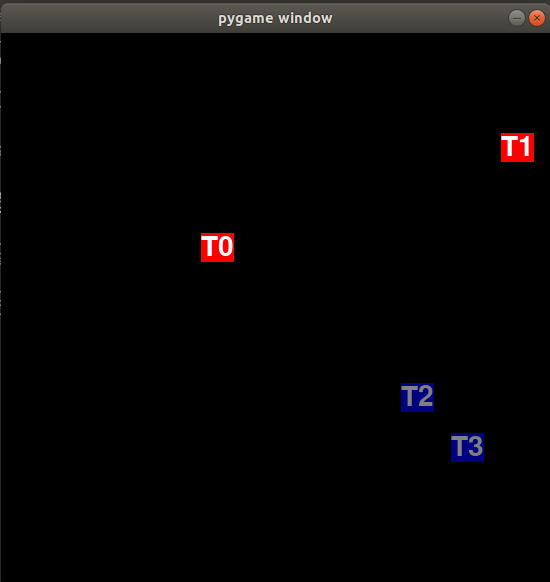
\includegraphics[scale=0.3]{images/game_visual.png}
\end{figure}
\end{frame}

\section{Results}
\begin{frame}{Independent RL}
\begin{columns}
\column{0.7\textwidth}
\begin{figure}[htp]
    \centering
    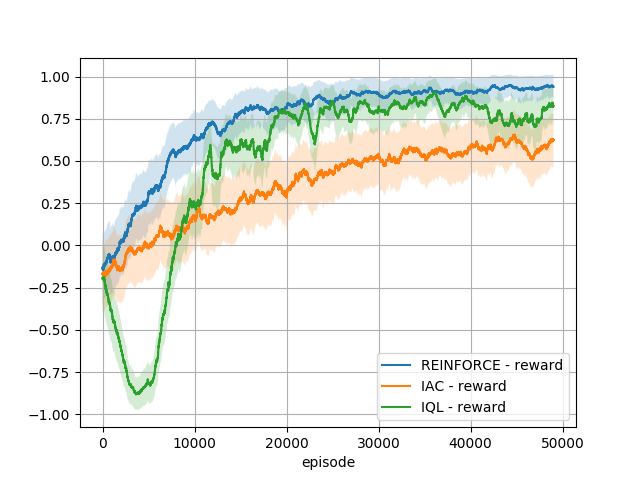
\includegraphics[width=\textwidth]{images/experiment4/compare_reward.png}
\end{figure}

\column{0.4\textwidth}
\begin{block}{Setup}
\begin{itemize}
    \item $2$ vs $2$
    \item Board: $7$-by-$7$
\end{itemize}
\end{block}
\begin{block}{Comparison}
\begin{itemize}
    \item REINFORCE is best
    \item IQL works but is lower and has higher variance
    \item IAC is inferior
\end{itemize}
\end{block}
\end{columns}
\end{frame}



\begin{frame}{QMix}
\begin{columns}
\column{0.7\textwidth}
\begin{figure}[htp]
    \centering
    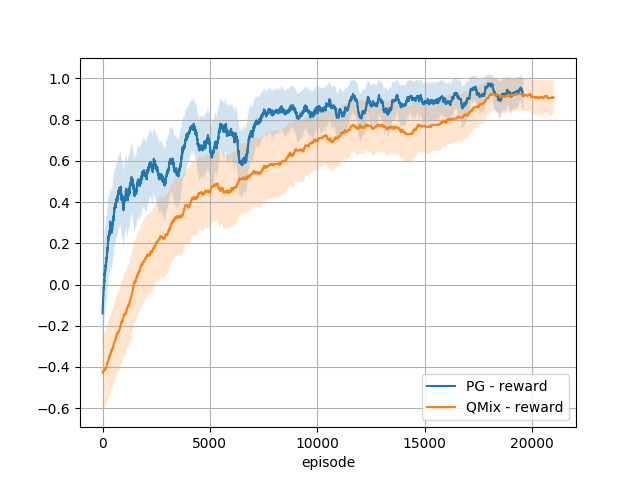
\includegraphics[width=\textwidth]{images/experiment6/qmix_vs_pg_win_9.png}
\end{figure}
\column{0.4\textwidth}
\begin{block}{Comparison}
\begin{itemize}
    \item QMix works quite well
    \item However, REINFORCE has better sample-efficiency
    \item QMix doesn't scale to larger board sizes
\end{itemize}
\end{block}
\end{columns}
\end{frame}

\begin{frame}{Model Transfer}
\begin{columns}

\column{0.5\textwidth}
\begin{block}{}
\begin{itemize}
    \item Playing against random agents is not that hard
    \item Idea:
        \begin{enumerate}
            \item Train for number of steps
            \item Transfer trained model to opponents
            \item Continue training against better opponents
        \end{enumerate}
    \item Finally, obtain strategy that also works against more intelligent opponents
\end{itemize}
\end{block}
\column{0.6\textwidth}
\begin{figure}[htp]
    \centering
    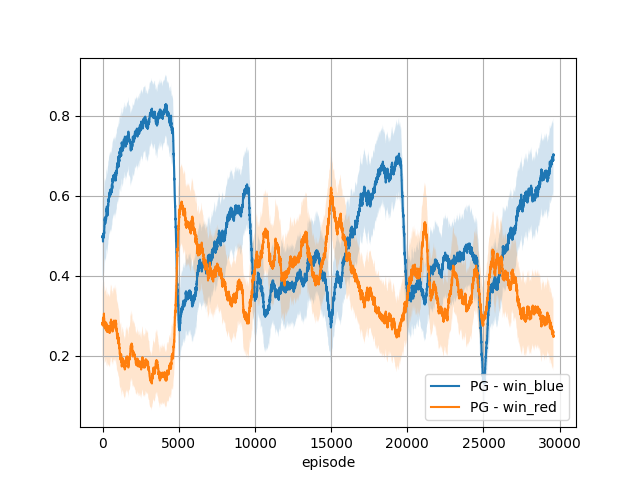
\includegraphics[width=\textwidth]{images/iteration/iterative.png}
\end{figure}

\end{columns}
\end{frame}

\begin{frame}{Game play - example 1}
\begin{columns}
\column{0.3\textwidth}
\begin{figure}[htp]
  \centering
  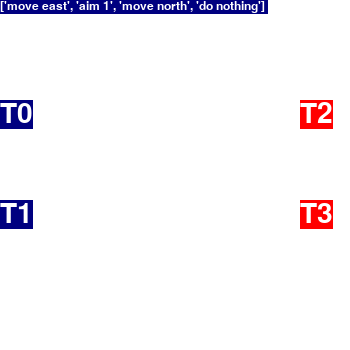
\includegraphics[width=\textwidth]{images/animation03/screenshot01.png}
\end{figure}
\begin{figure}[htp]
  \centering
  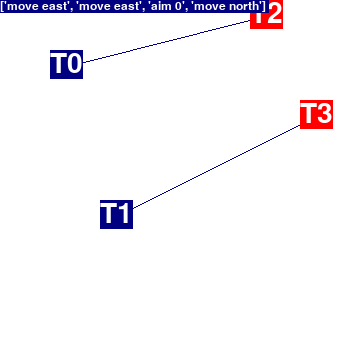
\includegraphics[width=\textwidth]{images/animation03/screenshot04.png}
\end{figure}

\column{0.3\textwidth}
\begin{figure}[htp]
  \centering
  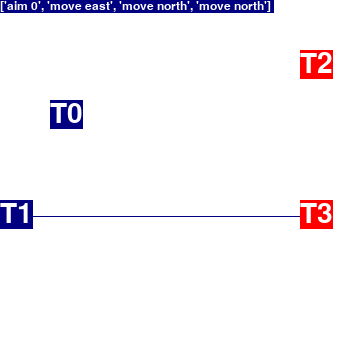
\includegraphics[width=\textwidth]{images/animation03/screenshot02.png}
\end{figure}
\begin{figure}[htp]
  \centering
  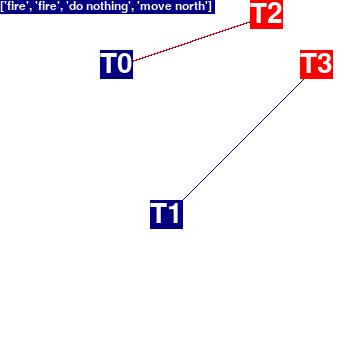
\includegraphics[width=\textwidth]{images/animation03/screenshot05.png}
\end{figure}

\column{0.3\textwidth}
\begin{figure}[htp]
  \centering
  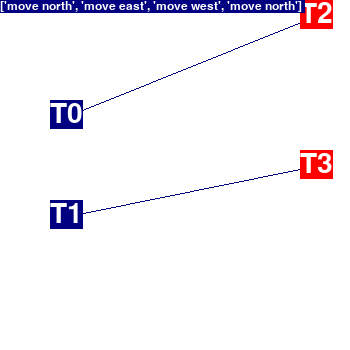
\includegraphics[width=\textwidth]{images/animation03/screenshot03.png}
\end{figure}
\begin{figure}[htp]
  \centering
  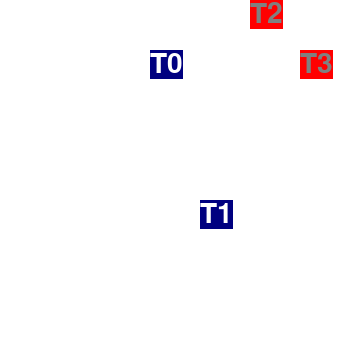
\includegraphics[width=\textwidth]{images/animation03/screenshot99.png}
\end{figure}

\end{columns}
\end{frame}

\begin{frame}{Game play - example 2}
\begin{columns}
\column{0.3\textwidth}
\begin{figure}[htp]
  \centering
  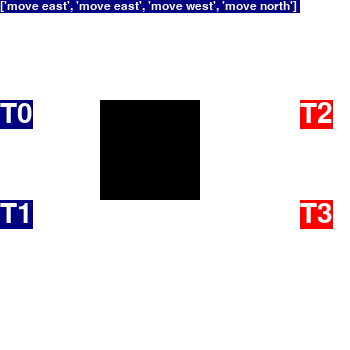
\includegraphics[width=\textwidth]{images/iteration/screenshot01.png}
\end{figure}
\begin{figure}[htp]
  \centering
  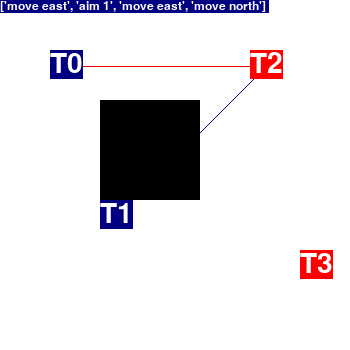
\includegraphics[width=\textwidth]{images/iteration/screenshot04.png}
\end{figure}

\column{0.3\textwidth}
\begin{figure}[htp]
  \centering
  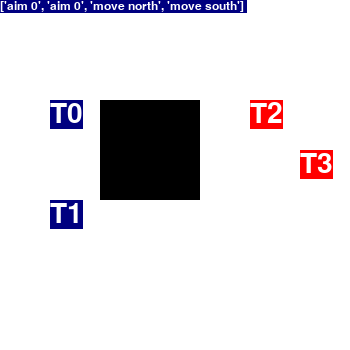
\includegraphics[width=\textwidth]{images/iteration/screenshot02.png}
\end{figure}
\begin{figure}[htp]
  \centering
  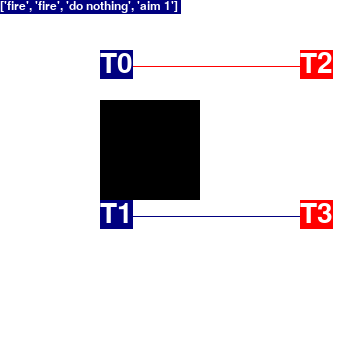
\includegraphics[width=\textwidth]{images/iteration/screenshot05.png}
\end{figure}

\column{0.3\textwidth}
\begin{figure}[htp]
  \centering
  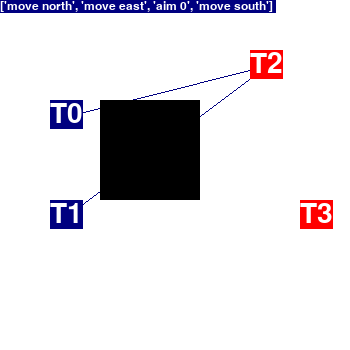
\includegraphics[width=\textwidth]{images/iteration/screenshot03.png}
\end{figure}
\begin{figure}[htp]
  \centering
  
\includegraphics[scale=0.5]{images/iteration/screenshot07.png}
\end{figure}

\end{columns}
\end{frame}

\section{Future Work}
\begin{frame}{Future Work}
\begin{block}{Problem is hard}
    \begin{itemize}
        \item \alert{Sparse rewards}: only at end of episode\\
               Solution: Reward shaping
        \pause
        \item \alert{Delayed rewards}: effect of good actions only later visible\\
              Solution: identify good actions, give them higher weight
        \pause
        \item \alert{Shared rewards}: which agent is responsible for win/loss?
        \pause
        \item \alert{Generalization}: opponents \& terrain
    \end{itemize}
\end{block}
    \pause
\begin{block}{Other improvements}
    \begin{itemize}
        \item Other network architecture
        \item Better (more realistic) model
        \item Other Multi-Agent algorithms
        \item Real-time ?
    \end{itemize}
\end{block}
\end{frame}

\section{Conclusions}
\begin{frame}{Conclusions}
\begin{block}{Modelling}
\begin{itemize}
    \item Algorithmic model of battlefield was developed
    \item This model is ready to be extended and to be made more realistic
\end{itemize}
\pause
\end{block}
\begin{block}{Algorithms}
\begin{itemize}
    \item A number of multi-agent RL algorithms have been explored
    \item Some of these algorithms give quite good results
    \item Others didn't live up to expectations
\end{itemize}
\end{block}
\pause
More research is needed:
\begin{itemize}
    \item Realistic models
    \item Better algorithms
    \item Feedback from people in the field
\end{itemize}
\end{frame}

\begin{frame}{Questions?}
\begin{center}
Thank you for your attention.\\
\Huge Any questions?
\end{center}
\end{frame}

\end{document}